\documentclass{beamer}
\newcount\tempcnt
\newcounter{temp}
\newtoks\temptoks
\newdimen\tempdim
\usetheme{chaoyang}
\usefonttheme{professionalfonts}
\usepackage[normalem]{ulem}
\usepackage{amsmath}
\usepackage[no-math]{fontspec}
\usepackage{xeCJK,unicode-math}
\setmainfont{Fira Sans}
\setsansfont{Fira Sans}
\setmonofont{FiraMono-Regular.otf}[
  BoldFont   = FiraMono-Bold.otf,
  ItalicFont = FiraMono-Oblique.otf,
  BoldItalicFont = FiraMono-BoldOblique.otf
]
\newfontfamily\lmmono{Latin Modern Mono}
\newfontfamily\cmuntt{CMU Typewriter Text}
\newfontfamily\stixtwo{STIX Two Text}
\newfontfamily\stixtwomath{STIX Two Math}
\setCJKmainfont{Source Han Sans SC}
\setCJKsansfont{Source Han Sans SC}
\setCJKmonofont{Source Han Sans SC Normal}
\setmathfont{Fira Math}
\usepackage{hyperref}
\hypersetup{hidelinks,psdextra}
\usepackage{minted}
\setminted{style=xcode,xleftmargin=.5em,fontfamily=tt}
\usepackage{array,graphicx,fonttable,tikz}
\usetikzlibrary{shapes,shapes.misc,calc}
\newcolumntype{z}{%
  >{%
    \hbox to 1em{\hss\ttfamily\tiny\textcolor{gray}{\the\tempcnt}}%
    \hskip.5em
    \special{color push rgb 0 0 0 }%
  }%
  w{l}{2.35em}%
  <{\special{color pop}\global\advance\tempcnt by 1}}
\makeatletter
\protected\def\textstar{{\stixtwomath\char"22C6}}
\DeclareRobustCommand\LaTeX{L\kern-.27em%
  {\sbox\z@ T%
   \vbox to\ht\z@{\hbox{\check@mathfonts
                        \fontsize\sf@size\z@
                        \math@fontsfalse\selectfont
                        A}%
                  \vss}%
  }%
  \kern-.1em%
  \TeX}
\DeclareRobustCommand\xelatex{X\kern-.125em\lower.5ex\hbox{\char"018E}%
  \kern-.125em\LaTeX}
\DeclareRobustCommand\pdflatex{pdf\LaTeX}
\DeclareRobustCommand\lualatex{Lua\LaTeX}
\DeclareRobustCommand\cs[1]{\texttt{\char`\\#1}}
\DeclareRobustCommand\meta[1]{$\langle\hbox{\itshape#1}\rangle$}
\DeclareRobustCommand\marg[1]{\texttt\{\meta{#1}\texttt\}}
\ExplSyntaxOn
\DeclareDocumentCommand \texfonttable { m O{\csname f@size\endcsname pt} }
  {
    \group_begin:
    \centering
    \tabcolsep = .25em
    \tex_font:D \l_temp_font_cs: = #1 ~ at ~ #2
    \cs_set:Npn \. ##1 { \texttt { \color { gray } \tiny ##1 } }
    \begin{tabular}{r|cccccccccccccccc}
      \hbox_to_wd:nn { 10pt } { } &
        \.0 & \.1 & \.2 & \.3 & \.4 & \.5 & \.6 & \.7 &
        \.8 & \.9 & \.A & \.B & \.C & \.D & \.E & \.F \\
      \hline
      \int_step_inline:nnn { 0 } { 7 }
        {
          \int_step_inline:nnn { -1 } { 15 }
            {
              \int_compare:nNnTF { ####1 } = { -1 }
                {
                  \.{ \texttt { \char`\" } ##1 $x$} &
                }
                {
                  {
                    \l_temp_font_cs:
                    \hbox_to_wd:nn { 12pt }
                      {
                        \tex_hss:D
                        \symbol { \int_eval:n { ##1 * 16 + ####1 } }
                        \tex_hss:D
                      }
                  }
                  \int_compare:nNnTF { ####1 } = { 15 }
                    {
                      \int_compare:nNnF { ##1 } = { 7 } { \\ }
                    }
                    { & }
                }
            }
        }
    \end{tabular}
    \tex_par:D
    \group_end:
  }
\ExplSyntaxOff
\makeatother

\title{字符编码与 \LaTeX{} 中的字体编码}
\author{AlphaZTX}
\date{2023/03/01}

\begin{document}
\maketitle

\begin{frame}
\section{字符编码}
\end{frame}

\begin{frame}{字符编码 (character encoding)}
\begin{exampleblock}{计算机如何读取“字符”?}\pause
\begin{itemize}%[<+->]
\item 计算机只能读取 0 和 1;
\item 计算机只能读取数字;
\item 将字符转写为数字;% 0 和 1 的序列;
\item 建立一个字符到数字的映射!
\end{itemize}
\end{exampleblock}
\end{frame}

\begin{frame}[fragile]{Examples}
\begin{exampleblock}{C}
\begin{minted}{c}
#include <stdio.h>
char foo = 65;
int main() {
    printf("%c", foo);
    return 0;
}
\end{minted}
\end{exampleblock}
\begin{exampleblock}{Python}
\begin{minted}{python}
foo = 65
print(chr(foo))
\end{minted}
\end{exampleblock}
\end{frame}

\begin{frame}[fragile]{Examples}
\begin{exampleblock}{Lua}
\begin{minted}{lua}
foo = 65
print(string.char(foo))
\end{minted}
\end{exampleblock}
\begin{columns}[t,totalwidth=\textwidth]
\begin{column}{.46\textwidth}
\begin{exampleblock}{\TeX\ (plain \TeX)}
\begin{minted}{tex}
\newcount\foo
\foo=65
\char\foo
\end{minted}
\end{exampleblock}
\end{column}
\hss
\begin{column}{.49\textwidth}
\begin{exampleblock}{\TeX\ (\LaTeX)}
\begin{minted}{latex}
\newcounter{foo}%
\setcounter{foo}{65}%
\symbol{\value{foo}}
\end{minted}
\end{exampleblock}
\end{column}
\end{columns}


\end{frame}

\begin{frame}{ASCII}% (1963)
\begingroup
\color{lightgray}\linespread{1.2}\lmmono
\tempcnt=32
\begin{tabular}{z|z|z|z|z|z|z|z}
\scalebox{.8}[1]{SP} & ! & \char`\" & \char`\# &
  \char`\$ & \char`\% & \char`\& & \char`\' \\
\hline
( & ) & \char`\* & + & , & - & . & / \\
\hline
0 & 1 & 2 & 3 & 4 & 5 & 6 & 7 \\
\hline
8 & 9 & : & ; & < & = & > & ? \\
\hline
@ & A & B & C & D & E & F & G \\
\hline
H & I & J & K & L & M & N & O \\
\hline
P & Q & R & S & T & U & V & W \\
\hline
X & Y & Z & [ & \char`\\ & ] & \char`\^ & \char`\_ \\
\hline
\char`\` & a & b & c & d & e & f & g \\
\hline
h & i & j & k & l & m & n & o \\
\hline
p & q & r & s & t & u & v & w \\
\hline
x & y & z & \char`\{ & \char`\| & \char`\} & \char`\~ & \scalebox{.6667}[1]{DEL}
\end{tabular}
\endgroup
\end{frame}

\begin{frame}{ASCII}
\begin{exampleblock}{Example}
\leavevmode\hbox to 3em{[SP]:\hss}%
\hbox to 6em{$32=2^5$\hss}→\quad$010\,0000\,\hbox{(bin)}$;\\
\leavevmode\hbox to 3em{A:\hss}%
\hbox to 6em{$65=2^6+1$\hss}→\quad$100\,0001\,\hbox{(bin)}$;
\end{exampleblock}
\end{frame}

\begin{frame}{Latin 1 (ISO/IEC 8859-1)}
\begingroup
\color{lightgray}\linespread{1.2}\lmmono
\tempcnt=160
\begin{tabular}{z|z|z|z|z|z|z|z}
\scalebox{.5}[1]{NBSP} & ¡ & ¢ & £ & ¤ & ¥ & ¦ & § \\
\hline
¨ & © & ª & « & ¬ & \scalebox{.6667}[1]{SHY} & ® & ¯ \\
\hline
° & ± & ² & ³ & ´ & µ & ¶ & · \\
\hline
¸ & ¹ & º & » & ¼ & ½ & ¾ & ¿ \\
\hline
À & Á & Â & Ã & Ä & Å & Æ & Ç \\
\hline
È & É & Ê & Ë & Ì & Í & Î & Ï \\
\hline
Ð & Ñ & Ò & Ó & Ô & Õ & Ö & × \\
\hline
Ø & Ù & Ú & Û & Ü & Ý & Þ & ß \\
\hline
à & á & â & ã & ä & å & æ & ç \\
\hline
è & é & ê & ë & ì & í & î & ï \\
\hline
ð & ñ & ò & ó & ô & õ & ö & ÷ \\
\hline
ø & ù & ú & û & ü & ý & þ & ÿ
\end{tabular}
\endgroup
\end{frame}

\begin{frame}{Latin 2 (ISO/IEC 8859-2)}
\begingroup
\color{lightgray}\linespread{1.2}\lmmono
\tempcnt=160
\begin{tabular}{z|z|z|z|z|z|z|z}
\scalebox{.5}[1]{NBSP} & Ą & ˘ & Ł & ¤ & Ľ & Ś & § \\
\hline
¨ & Š & Ş & Ť & Ź & \scalebox{.6667}[1]{SHY} & Ž & Ż \\
\hline
° & ą & ˛ & ł & ´ & ľ & ś & ˇ \\
\hline
¸ & š & ş & ť & ź & ˝ & ž & ż \\
\hline
Ŕ & Á & Â & Ă & Ä & Ĺ & Ć & Ç \\
\hline
Č & É & Ę & Ë & Ě & Í & Î & Ď \\
\hline
Đ & Ń & Ň & Ó & Ô & Ő & Ö & × \\
\hline
Ř & Ů & Ú & Ű & Ü & Ý & Ţ & ß \\
\hline
ŕ & á & â & ă & ä & ĺ & ć & ç \\
\hline
č & é & ę & ë & ě & í & î & ď \\
\hline
đ & ń & ň & ó & ô & ő & ö & ÷ \\
\hline
ř & ů & ú & ű & ü & ý & ţ & ˙
\end{tabular}
\endgroup
\end{frame}

\begin{frame}[fragile]{GBK}% 0x8140--0xFEFE
\begingroup\def\.#1{\texttt{\color{gray}\tiny#1}}%
\tabcolsep=.32em
\begin{tabular}{r|cccccccccccccccc}
\texttt{\color{gray}\footnotesize 81} &
  \.0 & \.1 & \.2 & \.3 & \.4 & \.5 & \.6 & \.7 &
  \.8 & \.9 & \.A & \.B & \.C & \.D & \.E & \.F \\
\hline
\.4 & 丂 & 丄 & 丅 & 丆 & 丏 & 丒 & 丗 & 丟 & 丠 & 両 & 丣 & 並 & 丩 & 丮 & 丯 & 丱 \\
\.5 & 丳 & 丵 & 丷 & 丼 & 乀 & 乁 & 乂 & 乄 & 乆 & 乊 & 乑 & 乕 & 乗 & 乚 & 乛 & 乢 \\
\.6 & 乣 & 乤 & 乥 & 乧 & 乨 & 乪 & 乫 & 乬 & 乭 & 乮 & 乯 & 乲 & 乴 & 乵 & 乶 & 乷 \\
\.7 & 乸 & 乹 & 乺 & 乻 & 乼 & 乽 & 乿 & 亀 & 亁 & 亂 & 亃 & 亄 & 亅 & 亇 & 亊 &    \\
\.8 & 亐 & 亖 & 亗 & 亙 & 亜 & 亝 & 亞 & 亣 & 亪 & 亯 & 亰 & 亱 & 亴 & 亶 & 亷 & 亸 \\
\.9 & 亹 & 亼 & 亽 & 亾 & 仈 & 仌 & 仏 & 仐 & 仒 & 仚 & 仛 & 仜 & 仠 & 仢 & 仦 & 仧 \\
\.A & 仩 & 仭 & 仮 & 仯 & 仱 & 仴 & 仸 & 仹 & 仺 & 仼 & 仾 & 伀 & 伂 & 伃 & 伄 & 伅 \\
\.B & 伆 & 伇 & 伈 & 伋 & 伌 & 伒 & 伓 & 伔 & 伕 & 伖 & 伜 & 伝 & 伡 & 伣 & 伨 & 伩 \\
\.C & 伬 & 伭 & 伮 & 伱 & 伳 & 伵 & 伷 & 伹 & 伻 & 伾 & 伿 & 佀 & 佁 & 佂 & 佄 & 佅 \\
\.D & 佇 & 佈 & 佉 & 佊 & 佋 & 佌 & 佒 & 佔 & 佖 & 佡 & 佢 & 佦 & 佨 & 佪 & 佫 & 佭 \\
\.E & 佮 & 佱 & 佲 & 併 & 佷 & 佸 & 佹 & 佺 & 佽 & 侀 & 侁 & 侂 & 侅 & 來 & 侇 & 侊 \\
\.F & 侌 & 侎 & 侐 & 侒 & 侓 & 侕 & 侖 & 侘 & 侙 & 侚 & 侜 & 侞 & 侟 & 価 & 侢 &    
\end{tabular}
\endgroup
\end{frame}

\begin{frame}[fragile]{Unicode}
\begingroup\def\.#1{\texttt{\color{gray}\tiny#1}}%
\tabcolsep=.32em
\begin{tabular}{r|cccccccccccccccc}
\texttt{\color{gray}\footnotesize 4E} &
  \.0 & \.1 & \.2 & \.3 & \.4 & \.5 & \.6 & \.7 &
  \.8 & \.9 & \.A & \.B & \.C & \.D & \.E & \.F \\
\hline
\.0 & 一 & 丁 & 丂 & 七 & 丄 & 丅 & 丆 & 万 & 丈 & 三 & 上 & 下 & 丌 & 不 & 与 & 丏 \\
\.1 & 丐 & 丑 & 丒 & 专 & 且 & 丕 & 世 & 丗 & 丘 & 丙 & 业 & 丛 & 东 & 丝 & 丞 & 丟 \\
\.2 & 丠 & 両 & 丢 & 丣 & 两 & 严 & 並 & 丧 & 丨 & 丩 & 个 & 丫 & 丬 & 中 & 丮 & 丯 \\
\.3 & 丰 & 丱 & 串 & 丳 & 临 & 丵 & 丶 & 丷 & 丸 & 丹 & 为 & 主 & 丼 & 丽 & 举 & 丿 \\
\.4 & 乀 & 乁 & 乂 & 乃 & 乄 & 久 & 乆 & 乇 & 么 & 义 & 乊 & 之 & 乌 & 乍 & 乎 & 乏 \\
\.5 & 乐 & 乑 & 乒 & 乓 & 乔 & 乕 & 乖 & 乗 & 乘 & 乙 & 乚 & 乛 & 乜 & 九 & 乞 & 也 \\
\.6 & 习 & 乡 & 乢 & 乣 & 乤 & 乥 & 书 & 乧 & 乨 & 乩 & 乪 & 乫 & 乬 & 乭 & 乮 & 乯 \\
\.7 & 买 & 乱 & 乲 & 乳 & 乴 & 乵 & 乶 & 乷 & 乸 & 乹 & 乺 & 乻 & 乼 & 乽 & 乾 & 乿 \\
\.8 & 亀 & 亁 & 亂 & 亃 & 亄 & 亅 & 了 & 亇 & 予 & 争 & 亊 & 事 & 二 & 亍 & 于 & 亏 \\
\.9 & 亐 & 云 & 互 & 亓 & 五 & 井 & 亖 & 亗 & 亘 & 亙 & 亚 & 些 & 亜 & 亝 & 亞 & 亟 \\
\.A & 亠 & 亡 & 亢 & 亣 & 交 & 亥 & 亦 & 产 & 亨 & 亩 & 亪 & 享 & 京 & 亭 & 亮 & 亯 \\
\.B & 亰 & 亱 & 亲 & 亳 & 亴 & 亵 & 亶 & 亷 & 亸 & 亹 & 人 & 亻 & 亼 & 亽 & 亾 & 亿  
\end{tabular}
\endgroup
\end{frame}

\begin{frame}{UTF-8}
\[\left\{
\vcenter{
\hbox to 9em{0--127\hss        ($2^7$)}
\hbox to 9em{128--2047\hss  ($2^{11}$)}
\hbox to 9em{2048--65535\hss($2^{16}$)}
}
\right.\]

\vskip1ex
\begin{exampleblock}{Example}
\begin{tabular}{c|rrr}
&Unicode
&\multicolumn{1}{c}{UTF-8}&\multicolumn{1}{c}{Bytes}\\
\hline
A  &    65 &                                     \texttt{\uline{0}1000001} & 1 \\
π  &   960 &                   \texttt{\uline{110}01111\,\uline{10}000000} & 2 \\
水 & 27700 & \texttt{\uline{1110}0110\,\uline{10}110000\,\uline{10}110100} & 3
\end{tabular}%
\end{exampleblock}
\end{frame}

\begin{frame}
\section{\LaTeX{} 中的字体编码}
\end{frame}

\begin{frame}{Character or glyph?}
\centering
\font\0="[lmroman10-regular.otf]"    at 24pt
\font\1="[lmroman10-italic.otf]"     at 24pt
\font\2="[lmroman10-bold.otf]"       at 24pt
\font\3="[lmroman10-bolditalic.otf]" at 24pt
\font\4="[lmsans10-regular.otf]"     at 24pt
\font\5="[lmsans10-oblique.otf]"     at 24pt
\font\6="[lmsans10-bold.otf]"        at 24pt
\font\7="[lmsans10-boldoblique.otf]" at 24pt
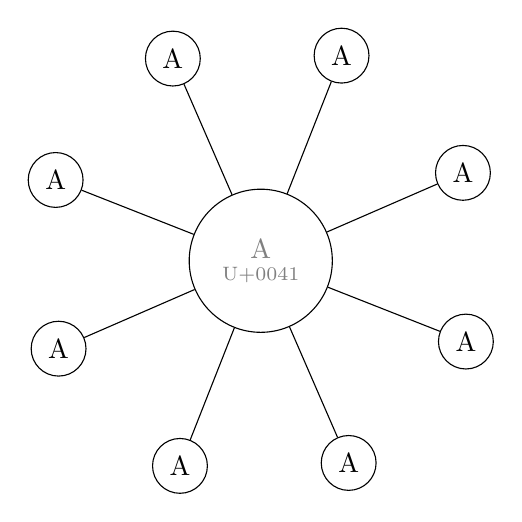
\begin{tikzpicture}
\node[circle,draw=black,text=gray] (O)
  {\vbox{%
    \hbox to 40pt{\hss\fontsize{48pt}{0pt}\lmmono A\hss}%
    \vskip-4pt
    \hbox to 40pt{\hss\scriptsize U+0041\hss}%
  }};
\foreach \i in {0,1,...,7}
  {
    \node[circle,draw] (\i) at ($(\i*45+23.5:2.8)$)
      {\csname\i\endcsname A\/};
    \draw (O) -- (\i);
  }
\end{tikzpicture}
\end{frame}

\begin{frame}[fragile]{Plain \TeX{} 内核预加载的字体}
\begin{exampleblock}{plain.tex}
\begin{minted}{tex}
\font\tenrm=cmr10  % roman text
\font\tensl=cmsl10 % slanted roman
\font\tenit=cmti10 % text italic
\font\tenbf=cmbx10 % boldface extended
\font\tentt=cmtt10 % typewriter
\font\teni=cmmi10  % math italic
\font\tensy=cmsy10 % math symbols
\font\tenex=cmex10 % math extension
% \font\preloaded=foo
% \let\preloaded=\undefined
\end{minted}
\end{exampleblock}
\end{frame}

\begin{frame}{cmr10 --- roman text}
\texfonttable{cmr10}
\end{frame}

\begin{frame}{cmbx10 --- boldface extended}
\texfonttable{cmbx10}
\end{frame}

\begin{frame}{cmti10 --- text italic}
\texfonttable{cmti10}
\end{frame}

\begin{frame}{cmmi10 --- math italic}
\texfonttable{cmmi10}
\end{frame}

\begin{frame}{cmsy10 --- math symbols}
\font\tempfont=cmsy10 at \csname f@size\endcsname pt%
\setbox0=\hbox{\tempfont\char"70}%
\tempdim=\dp0%
\vskip.54\tempdim%
\texfonttable{cmsy10}
\end{frame}

\begin{frame}{cmex10 --- math extensions}
\texfonttable{cmex10}[5.5pt]
\end{frame}

\begin{frame}{\LaTeX\ font encodings}
\begin{exampleblock}{Font encodings}
\makebox[2.5em][l]{\texttt{OT1}:}\TeX\ text\hfill ---cmr10, cmbx10, cmti10, etc;\\
\makebox[2.5em][l]{\texttt{OML}:}\TeX\ math italic\hfill ---cmmi10;\\
\makebox[2.5em][l]{\texttt{OMS}:}\TeX\ math symbol\hfill ---cmsy10;\\
\makebox[2.5em][l]{\texttt{OMS}:}\TeX\ math extension\hfill ---cmex10;\\
\makebox[2.5em][l]{\texttt{TU}:}\TeX\ Unicode\hfill ---OpenType;
\end{exampleblock}
\end{frame}

\begin{frame}{\LaTeX\ font encodings}
\centering

%\LaTeXe{} 字体命令
\cs{csname}%
\tikz[remember picture,inner sep=0pt,baseline=(currfontshape.base)]
  \node[black!60] (currfontshape) {\cs{curr@fontshape}};%
\texttt/%
\tikz[remember picture,inner sep=0pt,baseline=(fsize.base)]
  \node[black!60] (fsize) {\cs{f@size}};%
\cs{endcsname}%
\pause

\vskip2ex
{\color{lightgray}$\displaystyle\mathop{\overbrace{\hbox{\normalcolor%
\tikz[remember picture,inner sep=0pt,baseline=(fencoding.base)]
  \node[black!60] (fencoding) {\cs{f@encoding}};%
\texttt/%
\tikz[remember picture,inner sep=0pt,baseline=(ffamily.base)]
  \node[black!60] (ffamily) {\cs{f@family}};%
\texttt/%
\tikz[remember picture,inner sep=0pt,baseline=(fseries.base)]
  \node[black!60] (fseries) {\cs{f@series}};%
\texttt/%
\tikz[remember picture,inner sep=0pt,baseline=(fshape.base)]
  \node[black!60] (fshape) {\cs{f@shape}};%
}}}^{\hbox to 0pt{\hss
  \tikz[remember picture] \node[inner sep=0pt] (currfontshape2) {};%
\hss}}$}

\tikz[remember picture,overlay] \draw[-stealth,thick,out=270,in=90,cyBLOCKTblue]
  (currfontshape) to (currfontshape2);\pause

\vskip1ex
\texttt{\textbackslash}%
\tikz[remember picture,inner sep=0pt,baseline=(fencopt.base)]
  \node[gray] (fencopt)
  {$\begin{Bmatrix}
    \texttt{TU}\\ \texttt{OT1}\\ \texttt{OML}\\ \cdots
  \end{Bmatrix}$};%%
\texttt/%
\tikz[remember picture,inner sep=0pt,baseline=(ffamopt.base)]
  \node[gray] (ffamopt)
  {$\begin{Bmatrix}
    \texttt{cmr}\\ \texttt{lmr}\\ \texttt{ptm}\\ \cdots
  \end{Bmatrix}$};%
\texttt/%
\tikz[remember picture,inner sep=0pt,baseline=(fseropt.base)]
  \node[gray] (fseropt)
  {$\begin{Bmatrix}
    \texttt{m}\\ \texttt{b}\\ \texttt{bx}\\ \cdots
  \end{Bmatrix}$};%
\texttt/%
\tikz[remember picture,inner sep=0pt,baseline=(fshaopt.base)]
  \node[gray] (fshaopt)
  {$\begin{Bmatrix}
    \texttt{n}\\ \texttt{it}\\ \texttt{sl}\\ \cdots
  \end{Bmatrix}$};%
\texttt/%
\tikz[remember picture,inner sep=0pt,baseline=(fsizopt.base)]
  \node[gray] (fsizopt)
  {$\begin{Bmatrix}
  \texttt{10}\\ \texttt{7}\\ \texttt{5}\\ \cdots
  \end{Bmatrix}$};%
\pause

\tikz[remember picture,overlay]
  \draw[-stealth,thick,out=270,in=90,cyEXAMPLETgreen]
    (fencoding.south) to (fencopt.north);
\tikz[remember picture,overlay]
  \draw[-stealth,thick,out=270,in=90,cyEXAMPLETgreen]
    (ffamily.south) to (ffamopt.north);
\tikz[remember picture,overlay]
  \draw[-stealth,thick,out=270,in=90,cyEXAMPLETgreen]
    (fseries.south) to (fseropt.north);
\tikz[remember picture,overlay]
  \draw[-stealth,thick,out=270,in=90,cyEXAMPLETgreen]
    (fshape.south) to (fshaopt.north);
\tikz[remember picture,overlay]
  \draw[-stealth,thick,cyEXAMPLETgreen]
    (fsize.north) .. controls +(4,3) and +(4.5,2) .. (fsizopt.north east);

\end{frame}

\begin{frame}[fragile]{\LaTeX\ font encodings}
\begin{exampleblock}{Example}
\cs{OT1/cmr/m/n/10}\hfill\pdflatex\\
\cs{TU/lmr/m/n/10}\hfill\xelatex/\lualatex
\end{exampleblock}
\pause
\begin{exampleblock}{Plain \TeX\ version}
\begin{minted}{tex}
\expandafter\font
  \csname OT1/cmr/m/n/10\endcsname
    = cmr10 at 10pt
\end{minted}
\begin{minted}{tex}
\expandafter\font
  \csname TU/lmr/m/n/10\endcsname
    = "[lmroman10-regular]" at 10pt
\end{minted}
\end{exampleblock}
\end{frame}

\begin{frame}{\cs{OT1/cmr/m/n/10}\small\texttt{ = cmr10 at 10pt}}
\texfonttable{cmr10}
\end{frame}

\begin{frame}{\cs{TU/lmr/m/n/10}\small\texttt{ = "[lmroman10-regular]" at 10pt}}
\texfonttable{"[lmroman10-regular.otf]"}
\end{frame}

\begin{frame}{NFSS --- 用户接口}
\begin{exampleblock}{基本用户命令}
\begin{itemize}
\item \cs{fontencoding}\marg{encoding}
\item \cs{fontfamily}\marg{family}
\item \cs{fontseries}\marg{series}
\item \cs{fontshape}\marg{shape}
\item \cs{fontsize}\marg{size}\marg{baselineskip}
\item \cs{linespread}\marg{factor}\pause
\item[\hbox to 4pt{\hss\textstar\hss}] \textbf{\cs{selectfont}}\pause
\hfill{\color{gray}$\Rightarrow$ \cs{rmfamily}, \cs{mdseries}, \dots}\kern6pt
\end{itemize}
\end{exampleblock}
\end{frame}

\begin{frame}[fragile]{NFSS --- \cs{selectfont}}
\begin{exampleblock}{\cs{selectfont}}
\begin{enumerate}
\lineskiplimit4pt
\lineskip4pt
\item 设置行距:\cs{baselineskip}\;\texttt=\;\meta{factor}\cs{baselineskip};
\item 设置 shape 和 series;
\item 重定义 \cs{font@name} 并调用它;
\begingroup
\color{gray}\scriptsize
\begin{verbatim}
\xdef\font@name{%
  \csname\curr@fontshape/\f@size\endcsname}%
\pickup@font % 如果 \font@name == \relax,就重新定义一次
\font@name   % 切换字体
\end{verbatim}
\endgroup
\item \verb|\UseHook{selectfont}| (2021/06);
\item 更新暂时储存的 size 和 font encoding。
\end{enumerate}
\end{exampleblock}
\end{frame}

\begin{frame}{参考}
\begin{thebibliography}{9}
\bibitem{unicode}
  The Unicode standard.\newblock
  \href{https://www.unicode.org/versions/latest/}
       {\ttfamily unicode.org}
\bibitem{plain}
  \textit{Knuth D.}\enskip
  plain.tex (plain format kernel).\newblock
  \href{http://mirrors.ctan.org/macros/plain/base/plain.tex}
       {\ttfamily TDS:/tex/plain/base/plain.tex}
\bibitem{encguide}
  \textit{Mittelbach F.} and \textit{others}.\enskip
  \LaTeX\ font encodings.\newblock
  \href{http://mirrors.ctan.org/macros/latex/base/encguide.pdf}
       {\ttfamily texdoc encguide}
\bibitem{fntguide}
  \textit{\LaTeX\ Project Team}.\enskip
  \LaTeXe\ font selection.\newblock
  \href{http://mirrors.ctan.org/macros/latex/base/fntguide.pdf}
       {\ttfamily texdoc fntguide}
\bibitem{source2e}
  \textit{Braams J.} and \textit{others}.\enskip
  The \LaTeXe\ sources.\newblock
  \href{http://mirrors.ctan.org/macros/latex/base/source2e.pdf}
       {\ttfamily texdoc source2e}
\end{thebibliography}
\end{frame}

\end{document}